\section{Regularization}

When dealing with many candidates to use as covariates, one has to deal with the problem of selecting a subset of variables to use in constructing the model. 
This means that the vector of coefficients $\beta_\alpha = [ \beta_{1 \alpha} \cdots \beta_{P\alpha} ]$ should not have all nonzero values.
There are many ways of selecting a subset of variables among the available options.
Classical approaches for this problem are the Stepwise algorithm \cite{efroymson1960multiple}, \cite{hocking_selection_1967}, \cite{tibshirani1996regression}, which includes variables in sequence. 

Two approaches will be employed. At first, we use a Mixed Integer Linear Programming optimization problem (MILP) to find the best subset among all choices of covariates. The second way is by using a LASSO-type technique, which consists in penalizing the $\ell_1$-norm of regressors, thus shrinking the size of estimated coefficients towards zero.  

\subsection{Best subset selection via MILP}
\label{sec:best-subset-mip}

We use MILP to select variables by including constraints which limits their number in $K$. Only $K$ coefficients $\beta_{p\alpha}$ may have nonzero values, for each $\alpha$. 
Binary variable $z_{p\alpha}$ indicates whether $\beta_{p\alpha}$ has a nonzero value. 
The optimization problem that incorporates this idea is described below:
\begin{IEEEeqnarray}{lr}
\underset{\beta_{0\alpha},\beta_\alpha,z_{p \alpha}, \varepsilon_{t \alpha}^{+},\varepsilon_{t \alpha}^{-}}{\text{min}} \sum_{\alpha \in A} \sum_{t\in T}\left(\alpha\varepsilon_{t \alpha}^{+}+(1-\alpha)\varepsilon_{t\alpha}^{-}\right) \span \label{eq:mip0}  \\
\mbox{s.t } \span \nonumber \\
\varepsilon_{t \alpha}^{+}-\varepsilon_{t \alpha}^{-}=y_{t}-\beta_{0 \alpha}-\sum_{p=1}^{P}\beta_{p \alpha}x_{t,p}, \span \nonumber  \\
& \forall t \in T ,\forall \alpha \in A, \label{eq:mip1}  \\
\varepsilon_{t \alpha}^{+},\varepsilon_{t \alpha}^{-}\geq0, & \forall t \in T ,\forall \alpha \in A, \label{eq:mip2}\\
- M z_{p \alpha} \leq \beta_{p \alpha} \leq M z_{p \alpha}, & \forall \alpha \in A, \forall p\in P, \label{eq:mip3}\\
\sum_{p=1}^P z_{p \alpha} \leq K, & \forall \alpha \in A, \label{eq:mip4}\\
z_{p \alpha} \in \{0,1\}, & \forall \alpha \in A,  \forall p\in P, \label{eq:mip5}\\
\beta_{0\alpha} + \beta_{\alpha}^T x_{t} \leq \beta_{0\alpha'} + \beta_{\alpha'}^T x_{t},  \nonumber \\
\quad \qquad \qquad \forall t \in T, \forall (\alpha, \alpha') \in A \times A,  \alpha < \alpha', \span \label{eq:mip6}
\end{IEEEeqnarray}
%\begin{flalign}
%\underset{\beta_{0\alpha},\beta_\alpha,z_{p \alpha}, \varepsilon_{t \alpha}^{+},\varepsilon_{t \alpha}^{-}}{\text{min}} \sum_{\alpha \in A} \sum_{t\in T}\left(\alpha\varepsilon_{t \alpha}^{+}+(1-\alpha)\varepsilon_{t\alpha}^{-}\right) \span \span \label{eq:mip0}   \\
%\mbox{s.t } \nonumber \\
%& \varepsilon_{t \alpha}^{+}-\varepsilon_{t \alpha}^{-}=y_{t}-\beta_{0 \alpha}-\sum_{p=1}^{P}\beta_{p \alpha}x_{t,p}, \span  \label{eq:mip1} \\
%& &  \forall t \in T ,\forall \alpha \in A,  \nonumber\\
%& \varepsilon_{t \alpha}^{+},\varepsilon_{t \alpha}^{-}\geq0, & \forall t \in T ,\forall \alpha \in A, \label{eq:mip2}\\
%& - M z_{p \alpha} \leq \beta_{p \alpha} \leq M z_{p \alpha},& \forall \alpha \in A, \forall p\in P, \label{eq:mip3}\\
%& \sum_{p=1}^P z_{p \alpha} \leq K, & \forall \alpha \in A, \label{eq:mip4}\\
%& z_{p \alpha} \in \{0,1\}, & \forall \alpha \in A,  \forall p\in P, \label{eq:mip5}\\
%& \beta_{0\alpha} + \beta_{\alpha}^T x_{t} \leq \beta_{0\alpha'} + \beta_{\alpha'}^T x_{t}, \span \label{eq:mip6} \\
%& & \forall t \in T, \forall (\alpha, \alpha') \in A \times A,  \alpha < \alpha',   \nonumber
%\end{flalign}
The objective function and constraints (\ref{eq:mip1}), (\ref{eq:mip2}) and (\ref{eq:mip6}) are the same from standard linear quantile regression. 
By constraint (\ref{eq:mip3}), variable $z_{p \alpha}$ is a binary that assumes 1 when coefficient $\beta_{p \alpha}$ is included, while (\ref{eq:mip4}) guarantees that at most $K$ of them are nonzero.
The value of $M$ is chosen in order to guarantee that $M \geq \|\hat{\beta_\alpha}\|_{\infty}$. The solution given by $\beta_{0\alpha}^*$ and $\beta_\alpha^* = [ \beta_{1 \alpha}^* \cdots \beta_{P\alpha}^* ]$ will be the best linear $\alpha$-quantile regression with $K$ nonzero coefficients.  

\subsubsection*{Defining groups for variables}

Consider the optimization problem defined on (\ref{eq:mip0})-(\ref{eq:mip6}). The choice of the best subset is independent for different values of $\alpha$. This means that the best subset may include two completely different sets of regressors for two probabilities $\alpha$ and $\alpha'$ close to each other. Take $K=2$ for the example, selecting $\beta_{1\alpha}$ and $\beta_{4\alpha}$ for $\alpha$ while $\beta_{2\alpha'}$ and $\beta_{5\alpha'}$ is possible, but unlikely to be true.  

To address this issue, we propose to divide all $\alpha \in A$ in groups. The collection $G$ of all groups $g$ form a partition of $A$, and each $\alpha$ belongs to exactly one group $g$. 
The subset of selected covariates must be the same for all $\alpha$ in the same group $g$. To model these properties as constraints on problem (\ref{eq:mip0})-(\ref{eq:mip6}), we substitute constraint (\ref{eq:mip3}) for the following equations:
\begin{IEEEeqnarray}{lr}
z_{p \alpha g} := 2 - ( 1-z_{pg}) - I_{g\alpha}\span  \label{mipgrupzpa} \\
\sum\limits_{g \in G} I_{g\alpha} = 1, &\forall \alpha \in A,\label{eq:mipgrupa} \\
-Mz_{p \alpha g}  \leq  \beta_{p \alpha g} \leq M z_{p \alpha g}, \nonumber \\ 
& \forall p \in P, \forall \alpha \in A,  \forall g \in G,  \label{eq:mipgrupb} \\
I_{g\alpha}, z_{pg} \in \{0,1\}, & \forall p \in P,  \forall g \in G, \label{eq:mipgrupc}
\end{IEEEeqnarray}
%\begin{align} - DUAS COLUNAS
%z_{p \alpha g} := 2 - ( 1-z_{pg}) - I_{g\alpha}\span \span \label{mipgrupzpa} \\
%\sum\limits_{g \in G} I_{g\alpha} = 1, & \forall \alpha \in A,\label{eq:mipgrupa}& \\
%-Mz_{p \alpha g}  \leq  \beta_{p \alpha g} \leq M z_{p \alpha g}, \forall p \in P, \forall \alpha \in A,  \forall g \in G, \span \span \label{eq:mipgrupb} \\
%&I_{g\alpha}, z_{pg} \in \{0,1\},& \, \forall p \in P,  \forall g \in G, \label{eq:mipgrupc}
%\end{align}
on problem (\ref{eq:mip0})-(\ref{eq:mip6}).
where $G$ is a set of group index and $z_{pg}$ is a binary variable that equals 1 iff covariate $p$ is included on group $g$ and $I_{g\alpha}$ equals 1 iff probability $\alpha$ belongs to group $g$. 
Constraint (\ref{eq:mipgrupb}) forces that 
$$\text{if }z_{pg} = 0 \text{ and }I_{g\alpha} =1 \text{ then } \beta_{p \alpha = 0}. $$
Hence, if covariate $p$ belongs to group $g$, this covariate is not among group's $g$ subset of variables, than its coefficient must be equal to $0$, for that $\alpha$.
Note that variable $z_{p \alpha}$ behaves differently than when we are not considering groups. This means that if probability $\alpha$ belongs to group $g$ but variable $p$ is not selected to be among the ones of group $g$, than $\beta_{p\alpha}$ is zero.
Equation (\ref{mipgrupzpa}) defines $z_{p\alpha}$ to simplify writing. 


%\subsubsection*{Defining groups for variables where each group consists of probabilities in sequence}
%%
%Each groups $g \in G$, as defined on the last section, may be any combination of probabilities $\alpha$, such that they don't be in sequence. Figure \ref{fig:heatmap-exemplo-grupos} shows an example of 
%
%\begin{figure}
%	\centering
%	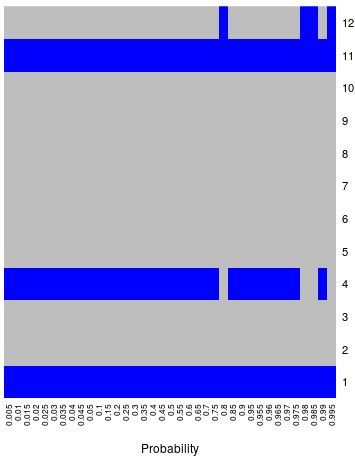
\includegraphics[width=0.4\linewidth]{Figuras/betas-mip/heatmap-exemplo-grupos}
%	\caption{}
%	\label{fig:heatmap-exemplo-grupos}
%\end{figure}
%
%
%\begin{eqnarray}
%\underset{\beta_{0\alpha},\beta_\alpha,z_{p \alpha}, \phi_{p \alpha}, \varepsilon_{t \alpha}^{+},\varepsilon_{t \alpha}^{-}}{\text{min}} & \sum_{\alpha \in A} \sum_{t\in T}\left(\alpha\varepsilon_{t \alpha}^{+}+(1-\alpha)\varepsilon_{t\alpha}^{-}\right) \label{eq:mipgr0} \\
%\mbox{s.t } & \varepsilon_{t \alpha}^{+}-\varepsilon_{t \alpha}^{-}=y_{t}-\beta_{0 \alpha}-\sum_{p=1}^{P}\beta_{p \alpha}x_{t,p},& \qquad\forall t \in T ,\forall \alpha \in A, \label{eq:mipgr1}\\
%& \varepsilon_{t \alpha}^{+},\varepsilon_{t \alpha}^{-}\geq0,&\qquad\forall t \in T ,\forall \alpha \in A, \label{eq:mipgr2}\\
%& - M z_{p \alpha} \leq \beta_{p \alpha} \leq M z_{p \alpha},&\qquad \forall \alpha \in A, \forall p\in\{1,\dots,P\}, \label{eq:mipgr3}\\
%& \sum_{p=1}^P z_{p \alpha} \leq K, & \qquad \forall \alpha \in A, \label{eq:mipgr4}\\
%& z_{p \alpha} \in \{0,1\},&\qquad \forall \alpha \in A, \forall p\in\{1,\dots,P\}, \label{eq:mipgr5}\\
%& \beta_{0\alpha} + \beta_{\alpha}^T x_{t} \leq \beta_{0\alpha'} + \beta_{\alpha'}^T x_{t}, & \qquad \forall t \in T, \forall (\alpha, \alpha') \in A \times A,  \alpha < \alpha',\nonumber\\ \label{eq:mipgr6} \\
%& z_{p\alpha} - z_{p\alpha+1} \leq m_{p\alpha}, & \qquad \forall \alpha \in A', \qquad \forall p \in P  \\
%& \sum_{\alpha \in A'} r_\alpha \leq |G| - 1 
%\label{eq:mipgr} \\
%\end{eqnarray}
%where $A' = A\setminus \{|A|\}$

\subsection{Variable selection via LASSO}
\label{sec:best-subset-ell1}

Another way of doing regularization is including the $\ell_1$-norm of the coefficients on the objective function. In \cite{belloni_l1-penalized_2009}, the reader can find properties and convergence rate when using the LASSO to select variables in a quantile regression setting. The ADALASSO variant is presented in \cite{ciuperca_adaptive_2016}. 
The advantage of this method is that coefficients are shrunk towards zero by changing a continuous parameter $\lambda$, which penalizes the size of the $\ell_1$-norm.  
When the value of $\lambda$ gets bigger, fewer variables are selected to be used. 
This is the same strategy of the LASSO methodology, and its usage for the quantile regression is discussed in \cite{li2012l1}.
The proposed optimization problem to be solved is:
\begin{equation}
\underset{\beta_{0\alpha},\beta_\alpha}{\text{min}} \sum_{t \in T}\alpha|y_{t}-q_\alpha(x_t)|^{+}+ \sum_{t \in T}(1-\alpha)|y_{t}-q_\alpha(x_t)|^{-}+\lambda\|\beta_\alpha\|_{1},
\label{eq:l1-qar-optim}
\end{equation}
\[
q_\alpha(x_t)=\beta_{0}-\sum_{p=1}^{P}\beta_{p}x_{t,p}.
\]

For such estimation to be coherent, however, each covariate must have the same relative weight in comparison with one another. 
So, before solving the optimization problem, we perform a linear transformation such that all variables have mean $\mu = 0$ and variance $\sigma^2 = 1$. 
We apply the transformation $\tilde{x}_{t,p} = (x_{t,p} - \bar{x}_{t,p}) / \hat\sigma_{x_{t,p}}$, where $\bar{x}_{t,p}$ and $\hat{\sigma}_{x_{t,p}}$ are respectively the sample's unconditional mean and standard deviation. The $\tilde{y}_{t-p,i}$ series will be used to estimate the coefficients, as this series has the desired properties. 

The process is done in two stages: variable selection and coefficients estimation. At first, all covariates are input on the following optimization problem:
\begin{IEEEeqnarray}{lr}
\tilde \beta_\lambda^{*LASSO} = \underset{\beta_{0},\beta,\varepsilon_{t \alpha}^{+},\varepsilon_{t \alpha}^{-}}{\text{arg min}} \sum_{\alpha \in A} \sum_{t \in T}(\alpha\varepsilon_{t \alpha}^{+}+(1-\alpha)\varepsilon_{t \alpha}^{-}) \span \nonumber \\
&  +\lambda\sum_{p=1}^{P}\mbox{\ensuremath{\xi}}_{p \alpha} \label{eq:obj-lasso} \\
\mbox{subject to } \nonumber & \\
\varepsilon_{t \alpha}^{+}-\varepsilon_{t \alpha}^{-}= y_{t}-\beta_{0 \alpha}-\sum_{p=1}^{P}\beta_{p \alpha}\tilde x_{t,p}, \span \nonumber \\
&\forall t\in T, \forall \alpha \in A, \\
\varepsilon_{t \alpha}^{+},\varepsilon_{t \alpha}^{-}\geq0,&\forall t \in T, \forall \alpha \in A,\\
\xi_{p\alpha}\geq\beta_{p \alpha},&\forall p\in P, \forall \alpha \in A,  \label{l1-qar-3}
\\
\xi_{p\alpha}\geq-\beta_{p \alpha},&\forall p\in P, \forall \alpha \in A.  \label{l1-qar-4}
\end{IEEEeqnarray}
This model is built upon the standard linear programming model for the quantile regression (\ref{eq:linear-opt-1})-(\ref{eq:linear-opt-ult}). 
On the above formulation, the $\ell_1$ norm of equation (\ref{eq:l1-qar-optim}) is substituted by the sum of $\xi_p$, which represents the absolute value of $\beta_{p\alpha}$. The link between variables $\xi_p$ and $\beta_{p\alpha}$ is made by constraints (\ref{l1-qar-3}) and (\ref{l1-qar-4}). Note that the linear coefficient $\beta_{0\alpha}$ is not included in the penalization, as the sum of penalties on the objective function \ref{eq:obj-lasso}.

% % % % % % % % Esse trecho deve ser usado quando os coeficientes do lasso forem utilizados, e não apenas o lasso sendo um seletor de variáveis % % % % % % % % %
%Each component of the output $\tilde \beta_\lambda^{*LASSO}$ must be corrected by multiplying each coefficient for its standard deviation: $\beta_{p\alpha,\lambda}^{*LASSO} = \tilde \beta_{p\alpha,\lambda}^{*LASSO} \hat\sigma_{x_{t,p}}$.
%\begin{eqnarray}
%\tilde \beta_\lambda^{*LASSO} = \underset{\beta_{0},\beta,\varepsilon_{t \alpha}^{+},\varepsilon_{t \alpha}^{-}}{\text{arg min}} & \sum_{\alpha \in A} \sum_{t \in T}\left(\alpha\varepsilon_{t \alpha}^{+}+(1-\alpha)\varepsilon_{t \alpha}^{-}\right)+\lambda\sum_{p=1}^{P}\mbox{\ensuremath{\xi}}_{p \alpha} \label{eq:obj-lasso} \\
%\mbox{subject to } & \varepsilon_{t \alpha}^{+}-\varepsilon_{t \alpha}^{-}= y_{t}-\beta_{0 \alpha}-\sum_{p=1}^{P}\beta_{p \alpha}\tilde x_{t,p},&\forall t\in T, \forall \alpha \in A, \\
%& \varepsilon_{t \alpha}^{+},\varepsilon_{t \alpha}^{-}\geq0,&\forall t \in T, \forall \alpha \in A,\\
%& \xi_{p\alpha}\geq\beta_{p \alpha},&\forall p\in P, \forall \alpha \in A,  \label{l1-qar-3}
%\\
%& \xi_{p\alpha}\geq-\beta_{p \alpha},&\forall p\in P, \forall \alpha \in A.  \label{l1-qar-4}
%\end{eqnarray}

For low values of $\lambda$, the penalty over the size of coefficients is small. Because of that, the output of problem (\ref{eq:obj-lasso})-(\ref{l1-qar-4}) is a model where most coefficients have nonzero value. On the other hand, when the penalty on $\| \beta_\alpha \|_1$ is big, many covariates will have zero valued coefficients. When $\lambda$ approaches infinity, one has a constant model. 
For instance, the penalty isn't applied to the linear coefficient $\beta_{0\alpha}$. 

In fact, the LASSO coefficients are biased, so it is employed only as a variable selector. 
The optimum vector of coefficients $\tilde \beta_\lambda{*LASSO}$ for a given $\lambda$ may be composed by both nonzero and zero coefficients. 
We then define $L_\lambda$ as the set of indexes of selected variables given by
\begin{equation*}
L_\lambda = \{ p \in \{ 1,\dots,P \} | \; |\beta^{*LASSO}_{\lambda,p}| \neq 0  \}.
\end{equation*}
Hence, we have that, for each $p \in \{ 1,\dots,P \}$,
$$\beta^{*LASSO}_{\lambda,p} = 0 \Longrightarrow \beta^{*}_{\lambda,p} = 0.$$

Note that problem (\ref{eq:linear-opt-1})-(\ref{eq:linear-opt-ult}) is employed to act as variable selection only. On the second stage, the optimal coefficient vector $\beta_\lambda{*LASSO}$ is estimated by the non-regularized QR, where only variables that bellongs to $L_\lambda$ are input:
\begin{IEEEeqnarray}{lC} (obj_{\lambda}^{*},\beta_{\lambda}^{*})\overset{(obj,var)}{\longleftarrow} \min_{\beta_0,\beta,\varepsilon_{t}^{+},\varepsilon_{t}^{-}} \sum_{t \in T} \left( \alpha \varepsilon_{t}^{+}+(1-\alpha) \varepsilon_{t}^{-}\right) \span \label{eq:post-lasso}
	 \\
\text{subject to } \span \nonumber \\
\varepsilon_{t}^{+}-\varepsilon_{t}^{-}=y_{t} - \beta_0 - \sum_{p\in L_\lambda} \beta_p x_{t,p},& \forall t\in T,\\
\varepsilon_t^+,\varepsilon_t^- \geq 0, & \forall t \in T.
\end{IEEEeqnarray}
The variable $obj_{\lambda}^{*}$ receives the value of the objective function on its optimal solution.
In summary, the optimization in equation \ref{eq:l1-qar-optim} acts as a variable selection for the subsequent estimation, which is normally called the post-LASSO estimation \cite{belloni2009least}.



% (\ref{eq:linear-opt-1})-(\ref{eq:linear-opt-ult}). 



